\chapter{Introduction}
\label{Introduction}

Audio processing, more precisely named audio signal processing, has been of interest since radio broadcasting and telephone systems capable of sound transmission started to replace the morse code\cite{spanias2006audio}. In it's simplest form, as used in the original telegraph, morse code is created by repeatedly opening an electrical circuit manually with a switch so that a visualisation device like a light bulb or an electric bell is turned on and off intermittedly. This discrete signal is transmitted over distance by extending the electrical circuit with long wires to a different physical location, so that the switch operator can transmit a message by morse encoding to the recipient who will have to use the same codebook for decoding.

\begin{figure}[h]
    \centering
	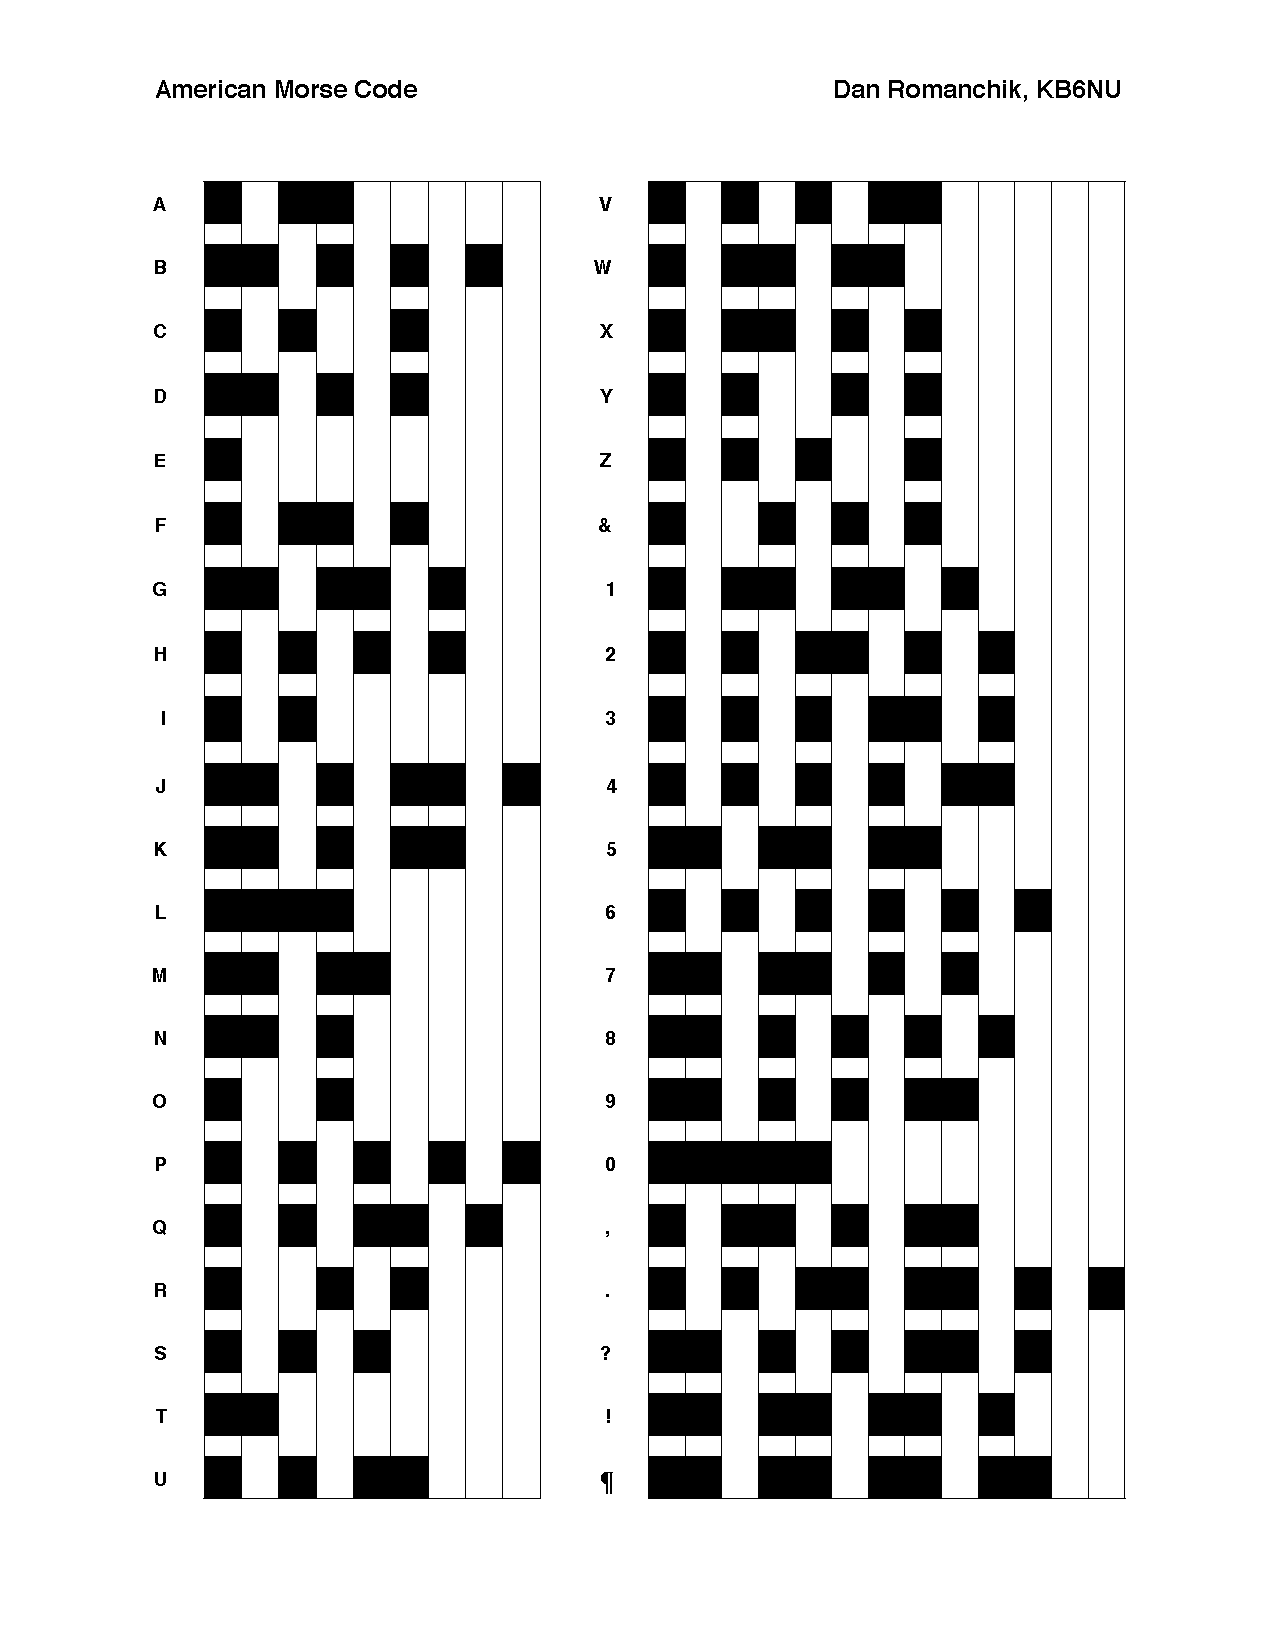
\includegraphics[width=.45\textwidth]{./images/illustrations/morse-chart}
    \caption{A codebook for the international morse code, where black means transmit}
    \label{fig:morse}
\end{figure}

The same purpose can be achieved wirelessly by repeatedly turning a radio transmitter on and off, which can be considered the simplest form of frequency modulation. However, things are more complex for the real- or near-time transmission of speech without manual en- and decoding. Since most harmonics of the human voice occur in the range of 500 Hz to 2 kHz according to the Nyquist–Shannon sampling theorem a sampling rate of at least 4 kHz is required for transmission\footnote{To verify this empirically I have downsampled a recording of both my voice and of the song Tom's Diner to 4kHz. While both the voice and the lyrics were still understandable, the melody perished and the sounds F and S were nearly indistiguishable. This is most like the reason why the common G.711 speech encoding standard uses a sampling rate of 8 kHz}. When radio transmission was invented in the late 19th century, it was not feasible to encode this information in a digital form (such as morse code). Instead different forms of modulation had to be developed, which was the birth of audio signal processing.

\begin{figure}[h]
    \centering
	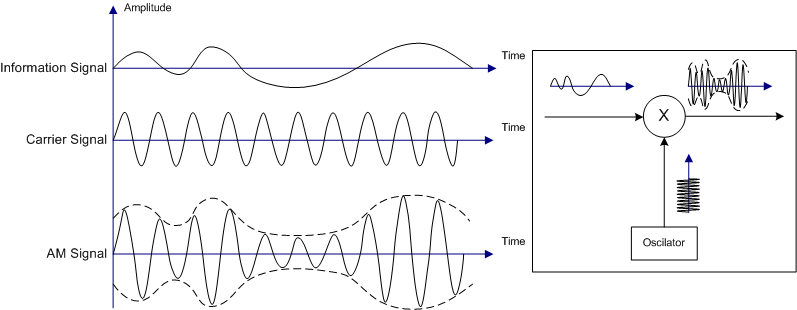
\includegraphics[width=.9\textwidth]{./images/illustrations/am}
    \caption{Amplitude modulation. Created by Ivan Akira. Source: CC-BY-SA; Wikipedia}
    \label{fig:am}
\end{figure}

 From the early 20th century onwards it started to transcended it's original use while still being required for every form telecommunication. The grammophone necessisated frequency alterations for more natural sound and the development of cinemas lead to improvements in speaker technology, separation of tweeter and woofer and required the invention of crossover networks\cite{spanias2006audio}.
 Today it is widely used for purposes such as entertainment (iPod), medical devices (ultrasound systems), magnetic storage of information (audio cassette, hard disks). 
 
 
  Before computers enabled digital signal processing, audio was handled via discrete analog circuits. An equalizer for example was constructed by using resonant circuits (consisting of an inductor and a capacitor) as a frequency filter to allow independent gain control with separate amplifiers for different bands. Audio processing consists of several different areas such as sound effects, modulation and demodulation, compression and quality enhancements like noise reduction.

An interesting area of audio processing is audio classification.  Given an audio sample, choose the best-fit class for that sample from a finite set of classes.  A common usage is music genre classification where the task is to find the genre a music sample belongs to. In this thesis my specifically focus is on urban sound classification: given an audio sample, choose which class, for example, shouting, car horns, or other sounds that occur in natural urban environments, the sample belongs to. This problem has several applications such as increasing the safety of self driving cars by detecting the existence and direction of car sirens before the car itself becomes visible or measuring the health impact of different forms of noise on the population.

The first project goal was to assist MIT AgeLab's human factors research in the traffic safety impact of self driving cars. This lab has a long history of detecting different forms of driver frustration with monitoring equipment in cars. They have also published research on the automatic detection of these factors through machine learning on video and audio\cite{Abdic:2016:DFD:3060621.3060809} instead of manual annotation.


\begin{figure}[h]
    \centering
	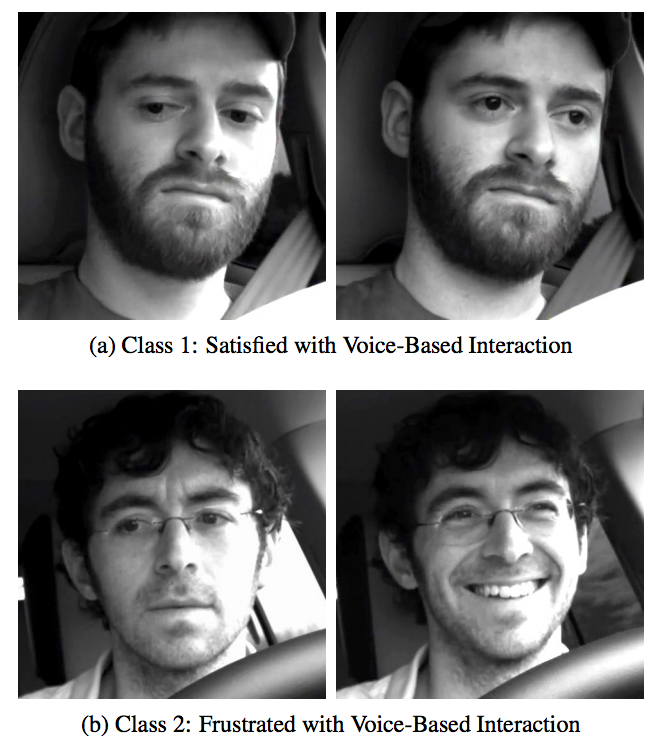
\includegraphics[width=.65\textwidth]{./images/illustrations/driver-frustration}
    \caption{Different examples of concentration and frustration while interacting with an in-car voice control system as shown in \cite{Abdic:2016:DFD:3060621.3060809}.}
    \label{fig:am}
\end{figure}

During this project software was created to automatically detect different sounds, most important the Tesla Autopilot's 'immediate takeover alarm`. I also attempted to use the developed detection of car horns to create a geogrpahic dataset of areas with high driver frustration and see if that could be correlated with accident statistics. However the available dataset of recorded traffic audio with position information turned out to be insufficient for this task.

Machine learning is especially interesting as an addition in the field of audio processing. Previously this has only seen popularity in the audio processing task of speech recognition. While there have been many advances in this area, there has been less work in other audio processing tasks, for example, in the detection of urban sounds and audio classification in general. Until recently, these tasks have been approached using sophisticated, hand-crafted features and algorithms that have existed since the sixties or earlier.  These algorithms were optimized to take advantage of analog hardware. As hardware advanced, more modern algorithms and techniques were able to be used such as gradient boosting and neural networks. These approaches represent the current state-of-the-art as it applies to audio classification.

The purpose of this thesis is to apply state-of-the-art neural network architectures and feature extraction to the task of urban sound classification using the UrbanSound8K dataset created by J. Salamon, C. Jacoby and J. P. Bello for the Sounds of New York City project \cite{Salamon:UrbanSound:ACMMM:14}. In this regard, I discuss several popular neural network architectures, such as CNNs, LSTMs, and attention mechanisms, and their performance in regards to audio classification. Specifically this thesis explores the use of LSTMs in urban sound classification, both with and without attention mechanisms. Furthermore, the results are compared to the use of gradient boosting and other existing algorithms against the same dataset.

\chapter{Background and Related Work}
\label{Background and Related Work}

Although there have been some recent breakthroughs in the field by Google's Deep Mind project (\cite{DBLP:journals/corr/OordDZSVGKSK16}) raw audio is rarely used  with machine learning algorithms directly. This is because one minute of mono channel audio, sampled with the very common AD conversion rate of 44.1 kHz, produces the amount of 2.646.000 data points alone. The data points are usually 16 bit integers indicating the amplitude of the audio wave at the present moment.


\begin{figure}[h]
    \centering
	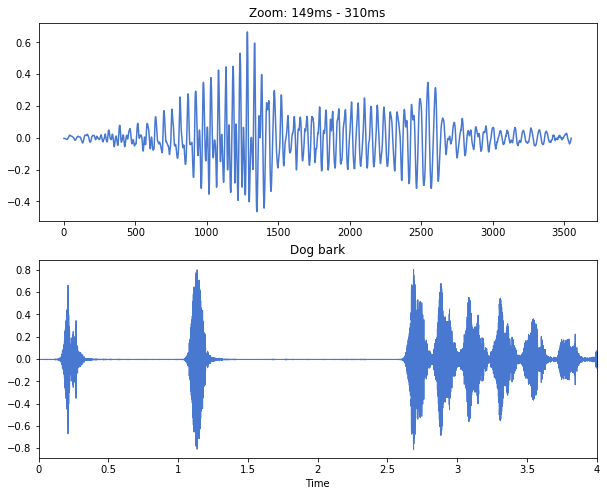
\includegraphics[width=.9\textwidth]{./images/illustrations/audio-signal}
    \caption{Common wave-plot representation of a 4s dog bark audio file and a zoom into seven 23ms frames consisting of 3549 data points}
    \label{fig:audio}
\end{figure}


This is in stark contrast to the amount of data in other machine learning tasks, such as the common 28x28 greyscale image in the MNIST image recognition dataset, where each image is represented by only $28*28*8 = 6.272$ bits \cite{lecun1998mnist}.

Therefor we rely on feature extraction through signal processing algorithms, that transforms the raw audio signal into meaningful information without removing the 


\section{Machine Learning for Audio through Feature Extraction}

For the purpose of this thesis, I have evaluated the ESSENTIA audio analysis library \cite{bogdanov:Essentia:ACMMULTIMEDIA13} via its Python bindings and librosa \cite{BMcFee:librosa}, a native python implementation. 
These have been selected as they seem to be the only actively-maintained open-source packages for audio signal processing with sufficient background literature and documentation. 

[wtd list and describe various audio processing task such as sound classification and speech recognition]

[wtd describe historical approaches to audio classification and audio processing tasks]

\subsection{Spectrograms}


\begin{figure}[h]
    \centering
	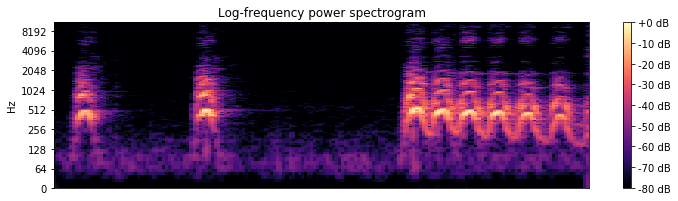
\includegraphics[width=.9\textwidth]{./images/illustrations/spectrogram}
    \caption{The spectral distribution of the dog bark audio}
    \label{fig:spef}
\end{figure}



\subsection{MFCC}

The most commonly used feature in speech recognition tasks are the Mel-frequency cep- stral coefficients (MFCCs)\cite{ganchev2005comparative}, a transformation that is inspired by the inner workings of the cochlea, including the sensory organ of hearing inside the human ear, the Organ of Cortil. The method has become extremely popular as it provides a separation between voice pitch and the formants \cite{noll67}. This is important in Indo- European languages where a change of the pitch usually does not alter a spoken word’s meaning \cite{auditoryneuroscience} and information is encoded by filtering the sound while passing the vocal tract, including the pharynx and the tongue causing changes in the envelope of the short time power spectrum.


\begin{figure}[h]
    \centering
	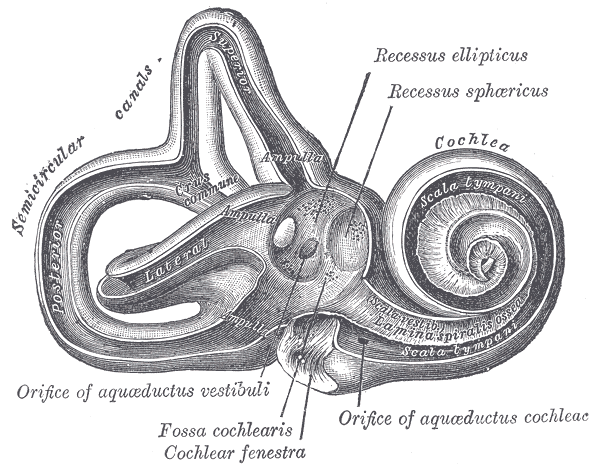
\includegraphics[width=.7\textwidth]{./images/illustrations/Gray921}
    \caption{Location and principle of the cochlea inside the inner ear. - Henry Gray, 1918, copyright expired}
    \label{fig:gray}
\end{figure}
s
The first step in its calculation is the slicing into short frames through a window function, mimicking inertia in the organ. Different sound frequencies create resonance in different areas of the cochlea’s narrowing spiral tube, where the wobbling of sensory hair called the stereocilia create nervous impulses. To identify the different frequencies, the next step is the calculation of a power spectrum through Fourier transformation. This result is a power spectrum on a linear frequency scale, which does not correlate well with the perception of different frequencies in humans \cite{mel}. While low frequencies below 20 Hz can hardly be detected, the effect becomes especially predominant with frequencies over 1 kHz. The transformation from the Hertz- onto the Mel-scale is used as the next step to map the spectrum onto the percieved frequencies. The linear scale is mapped into discrete bins through a triangular activation functions within the human hearing range as well in this step. Like most human senses in accordance to Fechner’s law \cite{fechner1860} the relationship between stimulus and perception is logarithmic, wich means a quadrupling of the acoustic pressure causes the perceived intensity (loudness) of sound to double. A similar effect can be achieved by taking the logarithms of the power spectrum. To decorrelate the energies of the overlapping filterbanks, in order to separate pitch, modulation (added by the vocal in human speech) and noise, the discrete cosine transformation is performed on the log mel powers. The resulting coefficient 2-13 form the MFCCs.


\section{Traditional machine learning approaches}
\subsection{Linear and Logistic Regression}

[wtd explain what it is, advantages such as linearly separable data, disadvatnages]

The primary downfall of linear/logistic regression is the inability to model non-linear relationships. [wtd explain this further]

\subsection{SVMs}


Support Vector Machine are among the most popular supervised machine learning methods. In its simplest form a model is created out of training data, with each instance belonging to one of two categories and the categories are linearly separable. The biggest improvement in SVMs over more traditional machine learning methods is, that it finds on optimal solution, and is not affected by local minima. Support vectors is the subset of data points that lie closest to the decision surface. These specify the decision function entirely by themselves. The SVM optimizes the margin around the separating hyper- plane (a line in 2 dimensional space) to be maximum. By using a kernel function, they can be extended onto categories that are not linearly separable. They can be used for classification as well as for regression.


Support vector machines (SVM) are... [wtd explain how support vector machines work].  SVMs have shown great success in the classification of high-dimensional data.

[wtd explain how kernel trick works]

[wtd, explain the what the pitfalls of SVMs are, such as choosing a kernel, citations needed]

\subsection{Random Forests}

[wtd explain how random forests work, include some math figures]

[wtd explain advantages of random forests, such as speed of training, higher accuracy on smaller dimensional data or datasets]

[wtd explain pitfalls of random forests]

\subsection{Gradient Boosting}

Gradient boosting is an supervised ensemble learning method that combines many "weak" learners, to form one single strong learner.  It has been proven to be a very successful machine learning method, has been applied with great success to many different Kaggle challenges (a machine learning competition).  It can be applied to both regression and classification problems.

[wtd explain gradient boosting, make sure to cite XGBoost and Adaboost papers]

[wtd explain advantages of gradient boosting]

[wtd explain disadvantages of gradient boosting]

\section{Neural Networks}

Contrary to the previously discussed approaches to machine learning, neural networks have existed for much longer [wtd cite Pitts and McCulloch the first neural network paper].  Neural networks have had a fickle history as well, with an ebb-and-flow of popularity, last peaking in the 90s [wtd cite some papers about NNs from Bengio, etc.].  Due to advances in computational power, parallel processing paradigms, and neural network architectures in the past several years, neural networks are seeing great successes across many machine learning tasks.  For example, in [wtd example task like MNIST or anything that had breakthrough results cite paper] neural networks were able to perform at a level previously thought not possible.  [wtd explain what neural networks are, put graphs, explain advantages such as ability to deal with curse of dimonsionality and ability to deal with non-linear relationships, explain pitfalls]. [wtd explain stochastic gradient descent and optimizers ADAM, Adadelta, momentum, etc.]

\subsection{Activation Functions}

After each neuron has calculated the sum of its weighted inputs, it passes it to a (usually non-linear) "activation" function.  There are advantages and disadvantages to different activation functions.


\subsubsection{Linear}

A linear activation function takes the weighted summed inputs to the neuron and multiplies it by a constant, giving the neuron the ability to scale the inputs.

{\centering
  $f(x)=cx$\par
}


\subsubsection{Sigmoid}
[wtd describe sigmoidal activation, include math]

{\centering
	$\displaystyle f(x)={\frac {L}{1+e^{-k(x-x_{0})}}}$\par
}

\subsubsection{TanH}

Similar to the sigmoid function, [wtd explain tanh]

\subsubsection{Rectified Linear Unit}
[wtd describe relu activation, include math]

{\centering
	$f(x)=max(0, x)$\par
}

\subsubsection{Scaled Exponential Linear Unit}
[wtd describe selu activation, include math, include special initialization required]


{\centering
	$\text{selu}(x) = \lambda\ \begin{cases}
    x,& \text{if } x > 0\\
    \alpha e^{x} - \alpha,& \text{if } x\leq 0\\
	\end{cases}$
	\par
}


The paper (\cite{DBLP:journals/corr/KlambauerUMH17})


\subsubsection{Softmax}
The softmax activation function transforms a set of probabilities

{\centering
	$\displaystyle \sigma (\mathbf {z} )_{j}={\frac {e^{z_{j}}}{\sum _{k=1}^{K}e^{z_{k}}}}$
	\par
}

\subsection{Convolutional Neural Networks}

Convolutional neural networks refers to any neural network with a convolutional layer.  These networks have achieved state-of-the-art results on many computer vision-related tasks, primarily because of their ability to "downsample" inputs while minimizing information loss.  It is because of this "downsampling" that these network are feasible to train, as opposed to a fully-connected network which has significantly more weights to train.  A convolutional layer is one that attempts to discover spatial relationships, aka filters, across neuronal inputs. [wtd describe + show graphs of convolutional layers].  This layer contains a set of filters, or weight matrices, that are convolved across the neuronal inputs, resulting in an output matrix called a feature map.  The weights of the filters are learned during training.  Typically these networks involve other spatial layers, such as max pooling layers, which directly downsample the neuronal inputs.

\subsection{Recurrent Neural Networks}

[wtd describe recurrent neural networks, cite original paper]

[wtd include math and graphs of basic RNN structure]

[wtd explain exactly the problem that RNNs solve (sequence and removing the need to include historical data in the inputs similar to how CNNs solve the problem of needing so many weights for the spatial input)]

While CNNS solve the problem of dimensionality in terms of spatial relationships, RNNs do so in terms of sequential, or temporal relationships.  Typically, to represent a temporal or sequential relationship, inputs are stacked in a windowed-fashion.  However, this greatly increases the number of weights required at the input layer.  Therefore, RNNs reduce the amount weights by allowing sequences to be passed in without requiring weights be connected to these input features.

\subsubsection{LSTMs}

\begin{figure}[h]
    \centering
	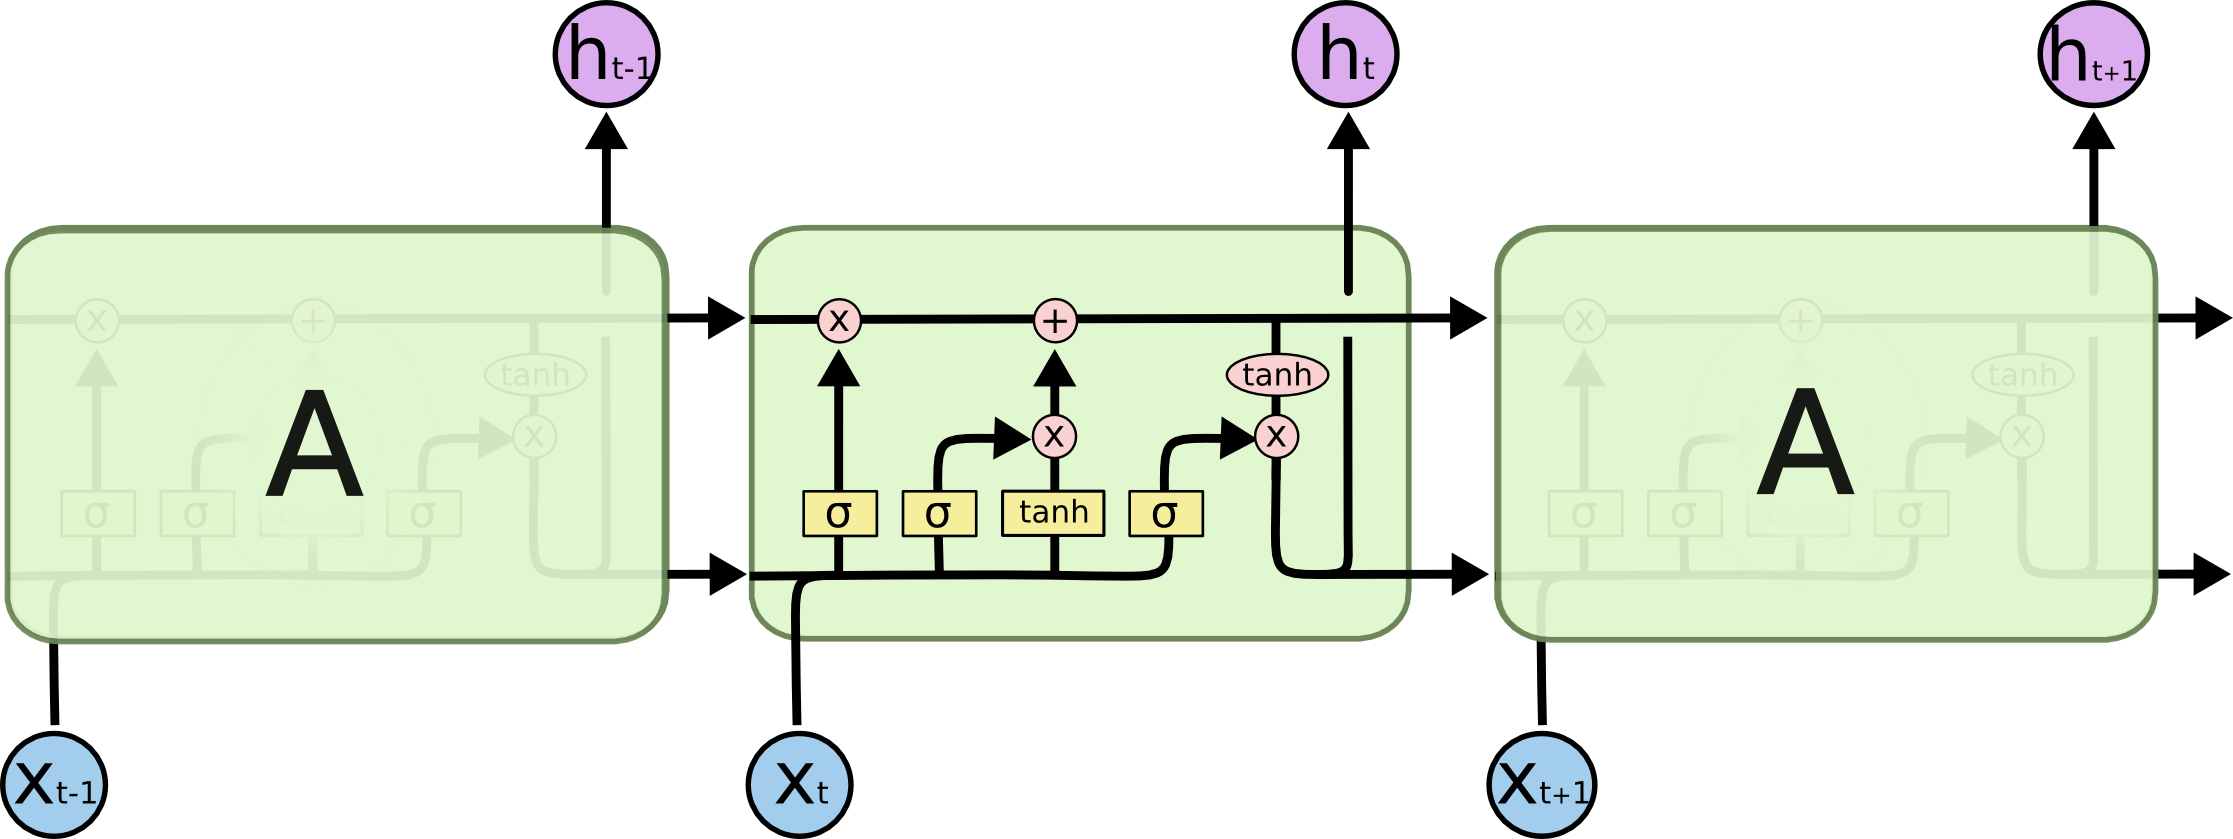
\includegraphics[width=.8\textwidth]{./images/illustrations/LSTM3}
    \caption{The repeating module in an LSTM contains four interacting layers.}
    \label{fig:mesh1}
\end{figure}\footnote{Source: http://colah.github.io/posts/2015-08-Understanding-LSTMs/. Reproduced with permission}





One of the pitfalls of recurrent neural networks is their inability to model [wtd describe lstms]

[wtd describe lstms and include graphs]

[wtd describe what problems lstms solve aka able to capture longer sequences, and downfalls]

\subsubsection{GRUs}

\begin{figure}[h]
    \centering
	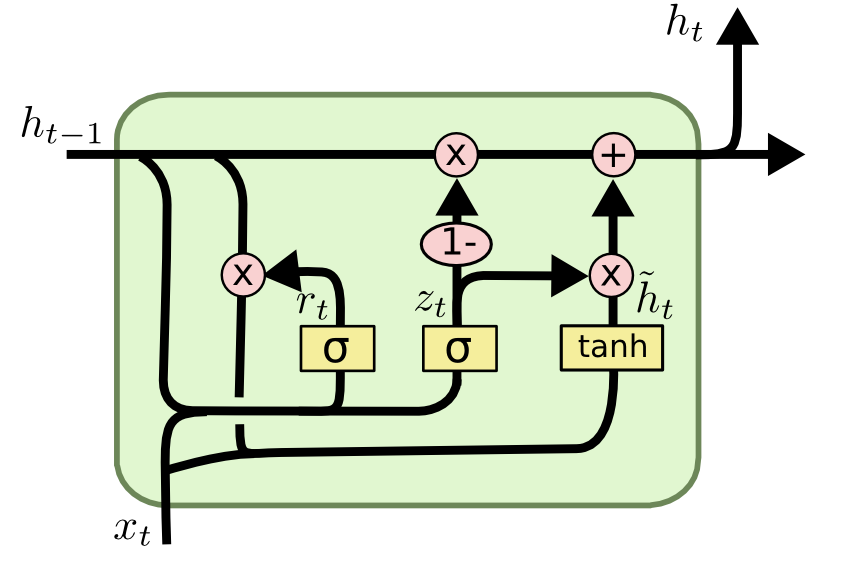
\includegraphics[width=.8\textwidth]{./images/illustrations/GRU}
    \caption{A GRU, as defined by Cho, et al. (2014).}
    \label{fig:mesh1}
\end{figure}\footnote{Source: http://colah.github.io/posts/2015-08-Understanding-LSTMs/. Reproduced with permission}



[wtd describe GRUs and include graphs]

[wtd describe what problems GRUs solve vs lstms vs RNNs, and downfalls]

\subsubsection{Attention Mechanisms}

[wtd describe attention mechanisms]

One of the more interesting recent discovering in the neural network architectures is that of attention mechanisms.  These approaches allow a neural network to "focus" on a specific area of input, and have produced state-of-the-art results in several machine learning tasks such as machine translation and speech recognition [wtd cite some papers on attention].

\subsection{Deep Learning}

One of the primary advances in neural networks in the past several years has been the advent of deep learning.  Existing conceptually since the inception of neural networks, deep learning refers to network architectures with more than one hidden layer.  Conventionally speaking, a deep network is a network with many hidden layers, sometimes in the hundreds [wtd cite microsoft paper on the 1000 layer network].  The discovery of adding more layers to a neural network to increase performance, however, has its own pitfalls.

For example, deep neural networks suffer from the problem of vanishing gradients [wtd cite some paper] and training time.  While previous approaches to conquering this problem have been somewhat successful [wtd cite bengio paper on how to actually train neural networks effectively], more advanced approaches have shown even greater success, for example normalization and regularization techniques, explained below.  Novel architectures such as deep residual networks [wtd cite microsoft deep residual network paper] have shown promise in this area as well.  Futhermore, the growing collection of larger annotated datasets and cheap, available processing power (such as GPUs and cloud computing), and the availability of open-source neural network toolkits have had major contributions to the success of neural networks as well [wtd cite tensorflow paper, torch, cite open source dataset papers].

\subsection{Recent Advances in Neural Networks}

Up until [wtd find the date of exploring weight initalization research] neural network weights were initialized randomly.  Contributing to the success of deep neural networks, several different initialization schemes have been discovered [wtd cite He initialization paper and other initializer papers, find these in the Keras documention]

For example, research into normalization and regularization has lead to faster training rates and higher accuracy, while preventing overfitting.  More specifically, batch normalization has shown to be greatly advantageous in speeding up the training of neural networks while reducing the amount of hyperparameter tuning [wtd cite batchnorm paper].  Batch normalization however, suffers from some issues [wtd pitfalls of batchnorm].

Even more recently, work has been done in the area of self-normalizing networks that [wtd cite SNN paper on SELU] remove the need for batch normalization and greatly increase accuracy and training speed in fully-connected neural networks.

\chapter{Dataset}

\section{Creation}

The UrbanSounds8K dataset used for this research is based on \cite{Salamon:UrbanSound:ACMMM:14}. It contains audio recording from the Freesound API, initially comprised 1302 recordings with the total length of 27 hours of audio and was manually labelled according to the Urban Sound Taxonomy created and introduced with the same paper. Labels span over 10 low-level classes in this taxonomy and offer an additional salience (foreground or background) classification.

The final audio samples have been provided by the authors publicly in the form of slices up to 4s long. Those were created by a 4s sliding window algorithm with a hop size of 2s and a limit of maximum 1000 slices per class. This results in a total of 8732 labeled slices or 8.75 hours of audio.

It is necessary to point out that the sliding window intentionally creates overlaps which result in the same audio information being present in up to two different slices. Additionally, due to the characteristics of urban sound, slices originating from the same original recording can have identifiable background or foreground sounds and other characteristics that can unintentionally be learned by the algorithm. %TODO: improve language

 This does not constitute a potenital for error, as long as 
  slices from the same source are not diverted across training and validation set. The authors provide for that by splitting the data into 10 distinct folds intended for k-fold cross validation as a means of model verification.

%TODO: Overlap -> overfit

We use the urban sound dataset SONYC, which is... [wtd put felix description of dataset here]. [wtd explain advantages of this dataset, explain pitfalls, dicusss other datasets and attempt to collect youtube horn dataset].  [wtd describe how it was created]

\section{Content}

As mentioned above, the dataset is labeled according to the Urban Sound Taxonomy(\cite{Salamon:UrbanSound:ACMMM:14}). The ten low-label classes present are air conditioner, car horn, children playing, dog bark, drilling, engine idling, gunshot, jackhammer, siren, and street music.

Unfortunately the occurences are unevenly distributed along the dataset, as shown in table \ref{tbl:urbansound8kdistribution}. 

\begin{table}[h]
\centering
\begin{tabular}{ll}
\hline
label & count \\
\hline
dog_bark & 1000 \\
children_playing & 1000 \\
car_horn & 429 \\
air_conditioner & 1000 \\
street_music & 1000 \\
gun_shot & 374 \\
siren & 929 \\
engine_idling & 1000 \\
jackhammer & 1000 \\
drilling & 1000
\end{tabular}
\caption{Amount of occurences per class in the UrbanSound8K dataset.}
\label{tbl:urbansound8kdistribution}
\par
\end{table}

The relatively low amount of car horns caused a problem, since the detection of various car horns was one of the AgeLab's main motivation.


\section{Feature Extraction}

As mentioned in the introduction, a raw audio signal consists of a high-dimensionality huge amount of data and is therefor not suitable as input for a learning algorithm without previous feature extraction.


% As noted in [13], the raw audio signal is not suitable as direct input to a classifier due to its extremely high dimensionality and the fact that it would be unlikely for perceptually similar sounds to be neighbours in vector space

% Thus, a popular approach for feature learning from audio is to convert the signal into a time-frequency representation, a common choice being the mel-spectrogram. We extract log-scaled mel-spectrograms with 40 components (bands) covering the audible frequency range (0-22050 Hz), using a window size of 23 ms (1024 samples at 44.1 kHz) and a hop size of the same duration. We alsoexperimented with a larger numbers of bands (128), but this did not improve performance and hence we stuck to the lower (and faster to process) resolution of 40 bands. To extract the mel-spectrograms we use the Essentia audio analysis library [20] via its Python bindings. Whilst we could use the resulting log-mel-spectrograms directly as input for the feature learning, it has been shown that the learned features can be significantly improved by decorrelating the input dimensions using e.g. ZCA or PCA whitening [18].

\subsection{Spectrogram}

\subsection{MFCC}

\subsection{Chroma}

\subsection{Quality improvements}
While usually not being succesful with neural networks, there has been moderate success in the classification of bird songs and acoustic scenes using more traditional classification methods like the spherical k-means algorithm in the past. To improve classification accuracy, \cite{Coates2012} has shown that dimensionality reduction with PCA whitening over scaled features has significatnly increased accuracy. 
This indicates that extracted features of a mel spectrogram are still heavily correlated.


[wtd describe what features are typically used in audio classification task]

[wtd describe what features were extracted by the SONYC team]

\chapter{Audio Classification using GRUs and Attention Mechanisms}

[wtd discuss implementation]

\section{Feature Engineering}

[wtd discuss what inputs were used, and how they were shaped]

[wtd discuss any additional preprocessing done]

\section{Network Architecture}

[wtd discuss exact nature of the architecture such as the layer, etc. include a graph, describe loss function]

\section{Training}

[wtd discuss batch sizes, number of epochs]

[wtd discuss train/test split, cross valdiation 10 fold?]

We evaluated training across several optimizers including SGD + momentum, Adam, and RMSProp.  Results for each optimizer are included in figure [wtd link to figure showing training times and loss]

For training and modeling the neural network, we used Python with the Tensorflow and Keras libraries [wtd include Keras/tensorflow citations].

The network was trained using a quad-core processor with an NVIDIA 1080 Ti graphics processer.

Overall, training took a total of [wtd include time of how long training took].

\section{Results}

[wtd results table]

Overall, we were able to achieve state-of-the-art results on the SONYC urban sound classification dataset using LSTMs with attention mechanism.

[wtd discuss pitfalls]

\chapter{Comparing Gradient Boosting to GRUs and Attention}

In addition to the deep neural network approach, we attempted to use gradient boosted trees, using the xgboost library [wtd cite xgboost] to achieve similar results.  As mentioned, gradient boosting has been very successful in classification tasks involving a small input dimensionality.

\chapter{Conclusion}

[wtd include results table of approaches to this dataset]

[wtd explain possible explanations for the results of our approach]

[wtd discuss problem with audio classification task]

We believe that one of the primary reasons audio classification is such a difficult task is due to the lack of available data.  Therefore, as the amount of labeled audio classification datasets increases (such as in genre classification [wtd cite stanford audio classification paper]), we predict there will be an increase in performance in this area.

